\chapter{Methodological Evolution}
\label{chap:methodological_evolution}

This chapter explains how the thesis methodology evolved from a broad search over possible planning approaches into a retained controller-centered thesis line, and why later solver-side work was still necessary even after that retained line had been established. The key point is that the final thesis method did not emerge as a single monolithic design chosen at the outset. Instead, the work progressed through a narrowing process. Early exploration considered a broader algorithmic space, including richer optimization formulations and multiple routing/control decompositions. The thesis then converged toward a controller-centered rolling-horizon line because that line offered the clearest experimental backbone, the strongest claim discipline, and the most reproducible paper-facing evidence. Only after that convergence did a second methodological transition occur: large-instance diagnostics revealed that some remaining failures were better interpreted as depot-wave execution bottlenecks, which motivated a more integrated controller-routing-repair architecture.

\section{Early methodological space}

At the start of the project, the methodological space was substantially broader than the final retained thesis line. The problem itself already combined several dimensions that each admit multiple solution traditions: rolling-horizon order admission, daily route construction under time windows and capacity constraints, multi-trip execution logic, and warehouse-side resource pressure. Taken together, these dimensions make it natural to consider a wide spectrum of approaches, ranging from exact or matheuristic formulations to simulation-driven controller design and scalable route heuristics.

In principle, one possible direction would have been to formulate the entire problem as a monolithic optimization model, combining cross-day service assignment, daily routing, trip structure, and depot-resource constraints in one large exact framework. Another possibility would have been to treat the work primarily as a routing-centered heuristic design problem, with warehouse pressure included only indirectly through penalties or post-hoc diagnostics. A third possibility would have been to place the emphasis on rolling decision policies, treating the daily routing backend as an execution module that supports higher-level admission and protection logic. The project initially remained open to all three interpretations.

This broader space was intellectually valuable, because it clarified the structural complexity of the thesis problem. The challenge is not just that routes are hard to build, nor just that future orders are uncertain. Rather, the difficulty lies in the interaction between flexible service-day control, same-day route feasibility, and resource usage that can spike sharply in short warehouse time buckets. In other words, the project began from a rich optimization perspective in which many method families were plausible. The final thesis method therefore should not be read as an arbitrary implementation choice, but as the outcome of a deliberate narrowing process.

A useful way to summarize the early method landscape is as a tension between breadth and thesis viability. Broader formulations promised stronger modeling completeness, but they also made it harder to maintain a clean experimental story and a defendable scope. Conversely, a narrower rolling-horizon controller line offered less immediate modeling breadth, but much greater clarity about what was being improved, how it should be evaluated, and which claims could be defended safely in a thesis setting. That tension is what ultimately drove the methodological narrowing described in the next section.

\section{Why the thesis narrowed to a controller-centered retained line}

The thesis narrowed toward a controller-centered retained line for four main reasons: reproducibility, evidence clarity, interpretable mechanism progression, and paper-facing claim discipline. These considerations mattered not only academically, but also practically. A graduation thesis needs more than a promising algorithmic idea; it needs a method line whose variants can be compared consistently, whose endpoint can be defended, and whose narrative does not depend on unstable or weakly interpretable branches.

First, the controller-centered line provided a clear rolling-horizon decision logic. It addressed the operational question of which visible orders should be admitted, protected, or deferred on each day, without requiring the entire contribution to hinge on one large and fragile route-level search mechanism. This made the cross-day planning role of the thesis explicit. Rather than treating daily routing as the only optimization object, the retained line treated admission and service prioritization as first-class design choices.

Second, this line produced an experimentally clean progression. Within the retained thesis scope, the main comparative chain could be written as \texttt{v2} $\rightarrow$ \texttt{v4} $\rightarrow$ \texttt{v5} $\rightarrow$ \texttt{v6f} $\rightarrow$ \texttt{v6g}. That progression is not a random list of versions. It functions as a mechanism sequence in which each step answers a more specific planning question under the same broad pressure setting. The retained line therefore supports a disciplined paper-facing story: baseline conditions are established by \texttt{EXP00} and \texttt{EXP01}, then the \texttt{Scenario1} controller line explains how the rolling controller improves service and failure outcomes under pressure.

Third, the retained line came with stronger claim guardrails. The writing-control files developed around the \texttt{22.03controller\_line} workspace make explicit which variants are mainline, which are supplementary, and which are only counterexamples or historical branches. This is particularly important for a thesis with many experimental branches. Without such guardrails, it would be easy to overstate the role of exploratory variants or to blur the distinction between a final retained endpoint and a promising but non-canonical follow-up. By contrast, the retained line makes it possible to state clearly that \texttt{v6g} is the current paper-facing main candidate, that \texttt{v6f} serves as a mechanism transition, and that variants such as \texttt{v6b3}, \texttt{cap05}, or \texttt{automode} must be interpreted more cautiously.

Fourth, the controller-centered line fit the thesis writing process itself. Because the progression was stable and the experimental roles were well defined, it could serve as the paper-facing backbone around which chapters on experiments, results, and discussion could be organized. This is why the retained line is best understood not merely as an old implementation, but as the backbone of the thesis evidence structure. In the manuscript, \texttt{22.03controller\_line} therefore functions as the retained reference line: it supplies the final controller progression, the main experimental spine, and the safest language for paper-facing claims.

\section{Methodology I: Controller-centered rolling admission control}

The retained method line can be described as a controller-centered rolling-horizon planning framework in which the primary methodological lever is not route optimization alone, but daily admission and protection decisions. At each planning day, the controller evaluates the visible order pool and determines which orders should be prioritized for service, which should be protected against displacement, and which flexible orders should be clipped or deferred to preserve downstream feasibility.

Conceptually, the method rests on three ideas. The first is \emph{urgency-aware admission}. Orders nearing the end of their service window, or otherwise judged difficult to recover later, must receive elevated priority. The second is \emph{protected capacity logic}. Not all demand should compete symmetrically for today's execution resources; some orders need structural protection to prevent high-throughput but less urgent flex demand from crowding them out. The third is \emph{risk-aware flex control}. Even when an order is still flexible, serving it today may create disproportionate future or execution risk, so the controller should selectively clip such demand rather than maximizing short-term throughput blindly.

Within the retained progression, these ideas become increasingly structured. The earlier retained controller versions establish a service-improving rolling admission baseline. Later versions add stronger commitment logic, risk budgeting, and explicit execution-aware protection. In the paper-facing narrative, the key progression is that \texttt{v4} improves over the earlier failure-first logic through more disciplined event-driven commitment, \texttt{v5} strengthens the line via risk-budgeted control, \texttt{v6f} identifies the importance of execution-aware protection, and \texttt{v6g} closes the main retained line through deadline reservation. This progression is central to the thesis because it shows that improvements in service and failure outcomes do not arise from random heuristic tuning; they emerge from increasingly explicit rolling-horizon control of risk, urgency, and protected demand.

The role of the daily routing backend within this methodology is important but secondary. In the retained line, the routing layer functions as an execution module that must produce feasible daily plans for the orders admitted by the controller. It supports the controller-centered methodology, but it is not yet the primary carrier of novelty in the thesis narrative. This distinction is essential. The retained line should not be described as if it had already solved the full integrated warehouse-distribution problem. Its main methodological contribution is instead to show that admission control and rolling protection mechanisms can materially improve service performance under pressure.

This is also why the retained method remains the paper-facing backbone even after later integrated solver work was introduced. It is interpretable, experimentally disciplined, and aligned with the thesis writing map. In the manuscript, it therefore plays the role of \emph{Methodology I}: the first complete and defensible answer to the rolling-horizon admission problem posed by the thesis.

\section{What Methodology I solved well, and what remained unresolved}

Methodology I solved an important part of the thesis problem well. It established that rolling-horizon service performance can be improved substantially through better controller logic. In particular, it showed that a controller that understands urgency, protected demand, and execution-aware risk can outperform cruder admission policies under pressure. This matters because it confirms that the multi-day service problem is not merely a downstream routing issue. Cross-day decision quality is itself a central determinant of service outcomes.

The retained line also solved the thesis writing problem well. It produced a stable mainline progression, a clear endpoint, and a defensible set of claims. This is not a trivial achievement. In many research projects, the most sophisticated branch is not the branch that ultimately supports the clearest thesis. Here, the retained controller-centered line succeeded precisely because it was methodologically interpretable and experimentally clean.

However, Methodology I also left a key issue unresolved. Its main logic acts at the level of admission, reservation, and service protection, while the most difficult execution stress can be much more localized. In particular, controller-level smoothing does not automatically internalize the warehouse time profile induced by the route set that is ultimately constructed. A policy may reduce broad daily pressure and still leave highly concentrated bucket-level overload, especially when many departures compete for picking effort in the same early wave.

This limitation is not a failure of the retained line; rather, it defines the boundary of what the retained line was designed to solve. The controller-centered methodology is strong at deciding which demand should be admitted into today's planning set and which should be deferred. It is weaker at directly reshaping the fine-grained temporal structure of depot workload once route construction begins. Thus, the unresolved issue is not simply ``routing remains hard.'' The unresolved issue is more specific: depot-resource realism enters too late and too indirectly if the main method lever remains controller-level admission alone.

That boundary is precisely what later solver-side work helped expose more clearly. Large-instance diagnostics, especially on West, suggested that some remaining performance difficulties were better explained by time-localized depot waves than by broad admission pressure alone. Once that observation is made, the natural methodological next step is not to discard the retained controller line, but to ask whether the planning architecture itself should internalize depot-resource information more explicitly.

\section{Transition to an integrated solver perspective}

The transition to the integrated solver perspective begins from that diagnostic realization. If the dominant execution problem on difficult instances is a narrow and severe depot-wave bottleneck, then improving controller logic alone may not be enough. The planning system must also become better at translating depot-resource pressure into route-construction and repair decisions. This insight motivates the move toward a more explicit three-layer architecture consisting of a controller, a routing backend, and a depot-repair layer.

Importantly, this transition should not be read as a repudiation of the retained controller-centered line. The two lines serve different roles in the thesis. The retained controller line remains the paper-facing reference line because it provides the clearest evidence chain for rolling admission control under pressure. The newer fresh-solver line instead reframes the thesis main system as an integrated solver architecture. Its contribution is to make warehouse-distribution coupling more explicit, to introduce richer diagnostics, and to show how depot-aware signals can enter route construction and repair more directly.

This distinction matters for how the thesis should be read. The integrated solver line is not simply ``version 2'' of the retained line, and it should not be ranked as if both systems were identical solver variants on a single flat experimental basis. Rather, the retained line supplies the mature controller-centered reference language, while the integrated line sharpens the thesis understanding of architecture, execution realism, and depot-coupled solving. The two therefore coexist in the manuscript with different narrative roles: the first anchors the retained experimental story, and the second extends the methodological interpretation of what the problem structurally requires.

Figure~\ref{fig:role_split_schematic} summarizes this division of labor visually. It is included here because the methodological evolution of the thesis is easier to understand once the reader sees that the controller-centered line and the integrated solver line were preserved for different scientific purposes rather than merged into one flat model family.

\begin{figure}[tbp]
    \centering
    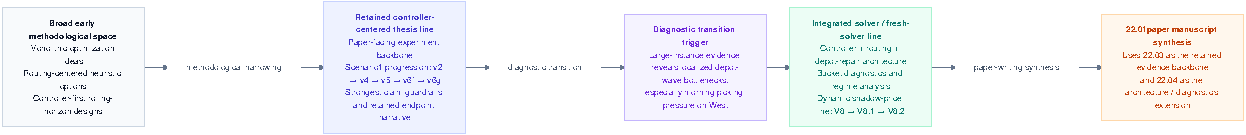
\includegraphics[width=0.98\textwidth]{Pictures/professor_preview/fig_role_split_schematic.pdf}
    \caption{Figure 4.1 shows the methodological evolution and role split in the thesis workspace. The project narrows from a broader early method space into the retained controller-centered thesis line, then transitions through depot-wave diagnostics into the integrated fresh-solver line. In the manuscript, \texttt{22.03controller\_line} remains the paper-facing evidence backbone, while \texttt{22.04fresh\_solver} contributes the architecture, diagnostics, and dynamic shadow-price mechanism extension.}
    \label{fig:role_split_schematic}
\end{figure}

This role split also serves as a writing guardrail. It explains why the retained line continues to anchor the paper-facing claims, while the fresh-solver line is used to deepen the architectural and diagnostic interpretation of the problem.

The next two chapters build on this transition. Chapter~\ref{chap:architecture_retained_method} shows how large-instance diagnostics lead to a more explicit integrated controller-routing-repair architecture. Chapter~\ref{chap:experimental_design} then presents the dynamic-shadow-price solver family that emerges within that integrated line. In this sense, the methodological evolution of the thesis is best understood as a two-stage narrowing. First, the project narrowed from a broad search space to a retained controller-centered thesis line. Second, that retained line exposed the need for a more explicit integrated architecture once depot-wave bottlenecks became analytically visible.
